\documentclass[tikz]{standalone}
\usepackage{amsmath}
\usepackage{times}
\usepackage{txfonts}

\usetikzlibrary{arrows}
\usetikzlibrary{intersections}
\usetikzlibrary{math}
\usetikzlibrary{positioning}
\usetikzlibrary{arrows.meta}
\usetikzlibrary{shapes.misc}
\usetikzlibrary{calc}

\begin{document}
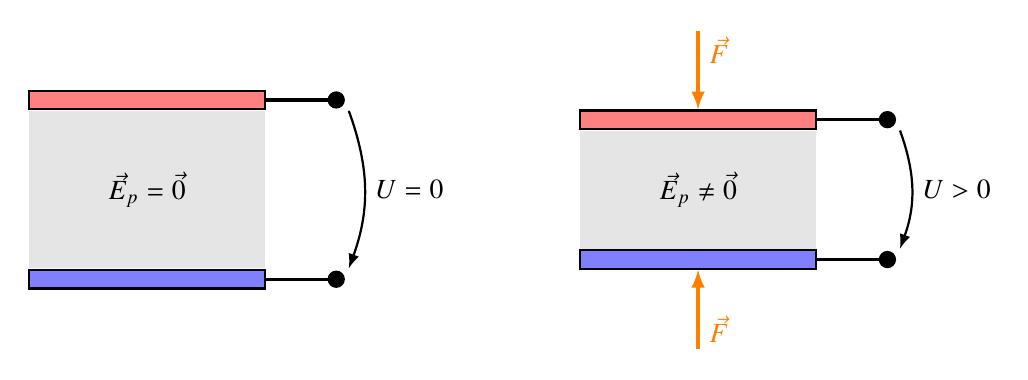
\begin{tikzpicture}[
    >=latex, 
  ]
  \begin{scope}[
        node distance = 0cm
    ]
    \node[
        rectangle, fill = gray!20!white,
        minimum width = 3cm, minimum height = 2cm,
    ] (body) {\(\vec{E}_p = \vec{0}\)};

    \node[
        draw, rectangle, thick, black, fill = red!50,
        minimum width = 3cm, minimum height = 1mm,
        above = of body
    ] (pos) {};

    \node[
        draw, rectangle, thick, black, fill = blue!50,
        minimum width = 3cm, minimum height = 1mm,
        below = of body
    ] (neg) {};

    \draw[black, very thick, -Circle] (pos.east) to ++ (1,0) node (p) {};
    \draw[black, very thick, -Circle] (neg.east) to ++ (1,0) node (n) {};

    \draw[black, thick, ->] (p) to[out = -70, in = 70] node[midway, right] {\(U = 0\)} (n);
  \end{scope}
  \begin{scope}[
        node distance = 0cm,
        xshift = 7cm
    ]
    \node[
        rectangle, fill = gray!20!white,
        minimum width = 3cm, minimum height = 1.5cm,
    ] (body) {\(\vec{E}_p \neq \vec{0}\)};

    \node[
        draw, rectangle, thick, black, fill = red!50,
        minimum width = 3cm, minimum height = 1mm,
        above = of body
    ] (pos) {};

    \node[
        draw, rectangle, thick, black, fill = blue!50,
        minimum width = 3cm, minimum height = 1mm,
        below = of body
    ] (neg) {};

    \draw[orange, very thick, <-] (pos.north) to node[near end, right] {\(\vec{F}\)} ++(0,1);
    \draw[orange, very thick, <-] (neg.south) to node[near end, right] {\(\vec{F}\)} ++(0,-1);

    \draw[black, very thick, -Circle] (pos.east) to ++ (1,0) node (p) {};
    \draw[black, very thick, -Circle] (neg.east) to ++ (1,0) node (n) {};

    \draw[black, thick, ->] (p) to[out = -70, in = 70] node[midway, right] {\(U > 0\)} (n);
  \end{scope}
\end{tikzpicture}
\end{document}
